%% abtex2-modelo-artigo.tex, v-1.7.1 laurocesar
%% Copyright 2012-2013 by abnTeX2 group at http://abntex2.googlecode.com/ 
%%
%% This work may be distributed and/or modified under the
%% conditions of the LaTeX Project Public License, either version 1.3
%% of this license or (at your option) any later version.
%% The latest version of this license is in
%%   http://www.latex-project.org/lppl.txt
%% and version 1.3 or later is part of all distributions of LaTeX
%% version 2005/12/01 or later.
%%
%% This work has the LPPL maintenance status `maintained'.
%% 
%% The Current Maintainer of this work is the abnTeX2 team, led
%% by Lauro César Araujo. Further information are available on 
%% http://abntex2.googlecode.com/
%%
%% This work consists of the files abntex2-modelo-artigo.tex and
%% abntex2-modelo-references.bib
%%

% ------------------------------------------------------------------------
% ------------------------------------------------------------------------
% abnTeX2: Modelo de Artigo Acadêmico em conformidade com
% ABNT NBR 6022:2003: Informação e documentação - Artigo em publicação 
% periódica científica impressa - Apresentação
% ------------------------------------------------------------------------
% ------------------------------------------------------------------------

\documentclass[
	% -- opções da classe memoir --
	article,			% indica que é um artigo acadêmico
	12pt,				% tamanho da fonte
	twoside,			% para impressão apenas no verso. Oposto a twoside
	a4paper,			% tamanho do papel. 
	% -- opções da classe abntex2 --
	%chapter=TITLE,		% títulos de capítulos convertidos em letras maiúsculas
	%section=TITLE,		% títulos de seções convertidos em letras maiúsculas
	%subsection=TITLE,	% títulos de subseções convertidos em letras maiúsculas
	%subsubsection=TITLE % títulos de subsubseções convertidos em letras maiúsculas
	% -- opções do pacote babel --
	english,			% idioma adicional para hifenização
	brazil,				% o último idioma é o principal do documento
	]{abntex2}


% ---
% PACOTES
% ---

% ---
% Pacotes fundamentais 
% ---
\usepackage{cmap}				% Mapear caracteres especiais no PDF
\usepackage{lmodern}			% Usa a fonte Latin Modern
\usepackage[T1]{fontenc}		% Selecao de codigos de fonte.
\usepackage[utf8]{inputenc}		% Codificacao do documento (conversão automática dos acentos)
\usepackage{indentfirst}		% Indenta o primeiro parágrafo de cada seção.
\usepackage{nomencl} 			% Lista de simbolos
\usepackage{color}				% Controle das cores
\usepackage{graphicx}			% Inclusão de gráficos
\usepackage{amsmath}			% amsmath
\usepackage{pdflscape}				% Páginas em formato paisagem
\usepackage{geometry}
\usepackage{hyperref}
\usepackage{listings}
%\usepackage{abntex2}
% ---
\graphicspath{{imagens/}}
% ---
% Pacotes adicionais, usados apenas no âmbito do Modelo C% ---
		
% ---
% Pacotes de citações
% ---
\usepackage[brazilian,hyperpageref]{backref}	 % Paginas com as citações na bibl
\usepackage[alf]{abntex2cite}	% Citações padrão ABNT
%\usepackage{natbib}
% ---

% ---
% Configurações do pacote backref
% Usado sem a opção hyperpageref de backref
\renewcommand{\backrefpagesname}{Citado na(s) página(s):~}
% Texto padrão antes do número das páginas
\renewcommand{\backref}{}
% Define os textos da citação
\renewcommand*{\backrefalt}[4]{
	\ifcase #1 %
		Nenhuma citação no texto.%
	\or
		Citado na página #2.%
	\else
		Citado #1 vezes nas páginas #2.%
	\fi}%
% ---

% ---
% Informações de dados para CAPA e FOLHA DE ROSTO
% ---
\titulo{Trabalho Prático 2 \\ Geração de Números Aleatórios}
\autor{Grupo 13 \\ Alisson Moreira Ferreira - 11/0106946 \\ Augusto Cesar Ribeiro Nunes - 13/0103004}
\local{Brasil}
\data{16 de abril de 2016}
% ---

% ---
% Configurações de aparência do PDF final

% alterando o aspecto da cor azul
\definecolor{blue}{RGB}{41,5,195}

% informações do PDF
\makeatletter
\hypersetup{
     	%pagebackref=true,
		pdftitle={\@title}, 
		pdfauthor={\@author},
    	pdfsubject={Trabalho Prático 2 da Disciplina Estatística Computacional 2},
	    pdfcreator={LaTeX with abnTeX2},
		pdfkeywords={abnt}{latex}{abntex}{abntex2}{atigo científico}, 
		colorlinks=true,       		% false: boxed links; true: colored links
    	linkcolor=blue,          	% color of internal links
    	citecolor=blue,        		% color of links to bibliography
    	filecolor=magenta,      		% color of file links
		urlcolor=blue,
		bookmarksdepth=4
}
\makeatother
% --- 

% ---
% compila o índice
% ---
\makeindex
% ---

% ---
% Altera as margens padrões
% ---
\setlrmarginsandblock{4cm}{4cm}{*}
\setulmarginsandblock{4cm}{4cm}{*}
\checkandfixthelayout
% ---

% --- 
% Espaçamentos entre linhas e parágrafos 
% --- 

% O tamanho do parágrafo é dado por:
\setlength{\parindent}{1.3cm}

% Controle do espaçamento entre um parágrafo e outro:
\setlength{\parskip}{0.2cm}  % tente também \onelineskip

% Espaçamento simples
\SingleSpacing

% ----
% Início do documento
% ----
\begin{document}

% Retira espaço extra obsoleto entre as frases.
\frenchspacing 

% ----------------------------------------------------------
% ELEMENTOS PRÉ-TEXTUAIS
% ----------------------------------------------------------

%---
%
% Se desejar escrever o artigo em duas colunas, descomente a linha abaixo
% e a linha com o texto ``FIM DE ARTIGO EM DUAS COLUNAS''.
% \twocolumn[    		% INICIO DE ARTIGO EM DUAS COLUNAS
%
%---
% página de titulo
\maketitle

% resumo em português
\begin{resumoumacoluna}
    Este Trabalho Prático implementa um gerador variáveis aleatórias Uniformes no intervalo (0,1) utilizando o Método Congruencial em (\ref{metodo:runif_cong}), implementa a geração de variáveis aleatórias Normais padrão utilizando o Método polar em (\ref{metodo:rnorm_polar}), e constrói uma tabela para as probabilidades acumuladas da N(0,1) utilizando duas implementações: o Método de Integração de Monte-Carlo em (\ref{tabela:pnorm_MC}) e a Probabilidade Acumulada Empírica obtida em (\ref{gerador:polar}) no item (\ref{tabela:pnorm_polar}). Os resultados são discutidos em \ref{cap:conclusoes}.
 
 \vspace{\onelineskip}
 
 \noindent
\end{resumoumacoluna}

% ]  				% FIM DE ARTIGO EM DUAS COLUNAS
% ---

% ----------------------------------------------------------
% ELEMENTOS TEXTUAIS
% ----------------------------------------------------------
\textual

% ----------------------------------------------------------
% Introdução
% ----------------------------------------------------------
\section{Introdução}
    Técnicas de Simulação são amplamente utilizadas em Ciências Naturais, Biológicas e na Tecnologia. Os seus custos diminuíram drasticamente nas últimas décadas, e acompanharam a evolução da computação em sentido inverso: hoje podemos simular processos com alto grau de sensibilidade e especificidade até mesmo em nossos computadores pessoais, e não mais em \textit{mainframes} cujo acesso era restrito e o custo elevadíssimo.
    
    Nas Ciências Físicas, podemos citar os sofisticados Modelos Climáticos \cite{ramirez2007desempenho} que utilizam simulação para a obtenção de previsões com maior ou menor grau de sucesso\footnote{O próprio \textit{paper} em questão faz uma espécie de meta-análise de modelos do IPCC, GFDL e HAD}. Na Estatística, a aplicação mais conhecida de Técnicas de Simulação são as ligadas direta ou indiretamente aos chamados \textbf{Métodos de Monte-Carlo}. 
    
    Na Estatística, encontramos aplicações (sofisticadas) de Simulação em Técnicas de Redução de Variância (como Amostragem de Importância e Amostragem Antitética) e em Processos Estocásticos (Algoritmo de Metropolis-Hastings, Amostragem de Gibbs, e MCMC). Em um nível mais simples, qualquer programa de computação científica que se preze contém uma implementação de geradores de variáveis aleatórias, um uso mais simples de Simulação.
    
    
\section{Metodologia}

    Este Trabalho Prático aborda em um de seus tópicos a Integração Numérica utilizando Monte-Carlo. A ideia é a seguinte: sendo $g(x)$ uma função arbitrária, e supondo que desejamos obter uma aproximação numérica para $\theta$ onde 
    
    \begin{equation}\label{eq:mc_01}
      \theta = \int_0^1g(x)dx  
    \end{equation}
    
    
    podemos olhar para $\theta$ como a Esperança de uma função $g(U)$ com $U \sim U(0,1)$. Supondo $U_1,\dots,U_n$ variáveis aleatórias independentes e identicamente distribuídas com $U_i \sim U(0,1)$ para $i = 1,\dots,n$, segue que $g(U_1),\dots,g(U_n)$ são variáveis aleatórias independentes e identicamente distribuídas com média $\theta$. Portanto, pela Lei Forte dos Grandes Números, temos com Probabilidade 1 que 
    
    \begin{equation}\label{eq:LFGN_MC}
        \lim_{n \rightarrow \infty}\sum_{i=1}^n\frac{g(U_i)}{n} \rightarrow E[g(U)] = \theta, 
    \end{equation}
    
    Logo, nós podemos aproximar $\theta$ utilizando uma amostra \textit{grande} de $u_i$ tirados de uma distribuição Uniforme em $(0,1)$. Para o caso mais geral onde os limites inferior e superior da integral (\ref{eq:mc_01}) são $a$ e $b$ quaisquer ($a<b$), podemos aplicar a substituição $y = (x-a)/(b-a), dy = dx/(b-a)$, obtendo 
    \begin{equation}\label{eq:MCI_arb}
        \theta = \int_0^1g(a+[b-a]y)(b-a)dy = \int_0^1h(y)dy
    \end{equation}
    
    onde $h(y) = (b-a)g(a+[b-a]y)$. Portanto, podemos aproximar $\theta$ tomando uma amostra de variáveis aleatórias Uniformes em $(0,1)$ e tomando a média de $h$ avaliada nas observações da amostra. A última parte do trabalho consiste na criação de uma tabela para a densidade acumulada da Normal(0,1), i.e., vamos aproximar a integral $\int_0^b \frac{1}{2\pi}exp\{-\frac{x_i}{2\sigma^2}\}$ utilizando o Método de Monte Carlo para integração numérica. O método foi implementado pela função \textbf{pnorm\_MC()}, e os valores obtidos com este método são comparados com os obtidos pela função \textbf{pnorm()} do R.
    
    Inicialmente há a necessidade de implementação de um gerador de variáveis aleatórias para a distribuição Uniforme em $(0,1)$. Utilizou-se o \textbf{Método Congruencial Multiplicativo} para tal finalidade. O método em questão consiste em, a partir de uma semente \textit{aleatória}\footnote{Na verdade, a maior parte os geradores aleatórios implementados e utilizados habitualmente são pseudo-aleatórios. Ver \cite{wiki:001} [em inglês] para uma explicação mais detalhada.}, obter uma sequência de números aleatórios ${x_1,x_2,\dots}$ tomando $x_n = (ax_{n-1}) \mod m$, com $a$ e $m$ inteiros positivos. Este gerador foi implementado pela função \textbf{runif\_congruencial()}. 
    
    Um outro método para geração de variáveis aleatórias estudado neste Trabalho Prático é o Método Polar\footnote{Em particular, utilizamos aqui o que se chama de Método Polar de Marsaglia: ver }: este método gera pares de variáveis aleatórias contínuas utilizando uma transformação em coordenadas polares. Em particular, implementamos um gerador de variáveis aleatórias Normais padrão, e sua função é \textbf{rnorm\_polar()}. Em um segundo momento, a distribuição acumulada empírica utilizando este método também foi utilizada para gerar uma tabela dos quantis da Normal padrão, comparando-a com os resultados da função \textbf{pnorm()} do R.
    
    As implementações, os resultados dos testes de hipóteses e sementes utilizados para verificar o ajustamento dos geradores encontram-se no Anexo A. As funções foram documentadas utilizando o pacote \textit{Roxygen} do R. Disponibilizamos um repositório no site github.com: \url{http://github.com/august-o/TP2-EstComp}. Lá encontram-se todos os arquivos-fonte utilizados neste Trabalho Prático. O computador utilizado foi um Macbook Pro, Sistema Operacional OS X El Capitan (10.11.3), com processador Intel Core i5 de 2.4 GHz e 16 GB de memória RAM 1333 MHz DDR3. A versão do R utilizada foi a 3.2.4, com a IDE RStudio em sua versão 0.99.1130.  
    
\section{Gerador Congruencial para a variável aleatória Uniforme(0,1)}\label{metodo:runif_cong}
\subsection{Teste de Uniformidade}
    Com a implementação adotada e a amostra obtida (ver Anexo A), foram realizados três Testes de Hipóteses para 
        
    \begin{align*}
        H_0 & : \mathbf{X} \sim U(0,1), (iid) \\
        H_1 & : \mathbf{X} \sim T
    \end{align*}
    
    onde \textbf{X} é o vetor aleatório  ($n = 10^5$) gerado pela implementação utilizada, e T é uma distribuição qualquer que não seja a Uniforme(0,1). O \textbf{Teste de Kolmogorov-Smirnov} para a Uniformidade da Distribuição gerada não rejeita a hipótese nula a um nível de significância de 0.7253, o \textbf{Teste de Cramér-von Mises} não rejeita a hipótese nula a um nível de significância 0.7823, e o \textbf{Teste de Anderson-Darling} não rejeita a hipótese nula a um nível de significância de 0.5601. 
    
    Como verificação qualitativa, adicional, abaixo estão os histogramas do vetor usando o gerador congruencial e do vetor utilizando \textbf{runif()} do R. Note que ambos são \textit{uniformes} e muito similares\footnote{Isso é o máximo que se pode dizer numa inspeção visual para "verificar" esse tipo de similaridade.}

    \begin{figure}[h]
        \centering
        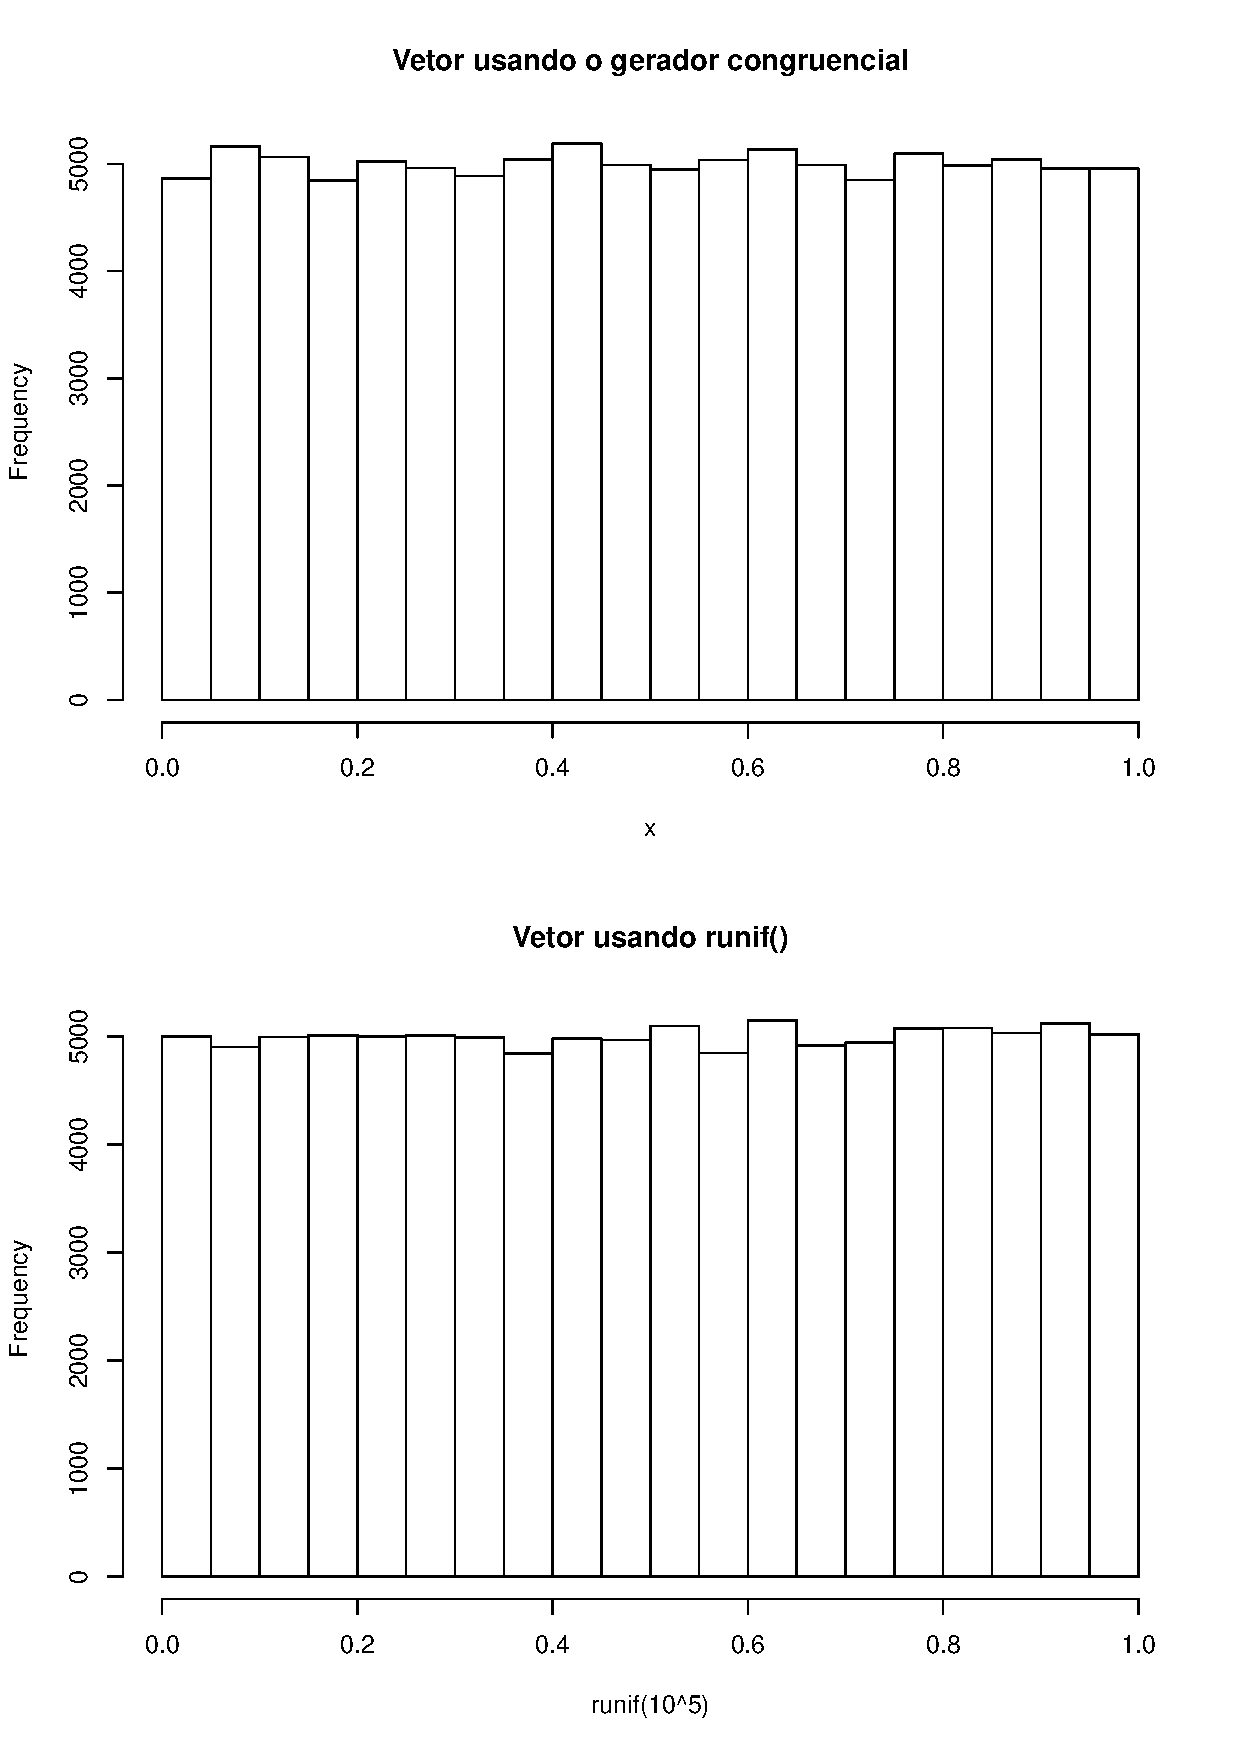
\includegraphics[scale=0.55]{hist_runif_congruencial}
        \caption{Histogramas para o gerador e para a função runif(), $n = 10^5$}
        \label{fig:hist_runif}
    \end{figure}
    
    \newpage
    
\section{Gerador Polar para a variável aleatória Normal Padrão}\label{gerador:polar}
\subsection{Teste de Normalidade}\label{metodo:rnorm_polar}
    Com a implementação adotada e a amostra obtida (ver Anexo A), foram realizados três Testes de Hipóteses para 
        
    \begin{align*}
        H_0 & : \mathbf{X} \sim N(0,1), (iid)\\
        H_1 & : \mathbf{X} \sim T
    \end{align*}
    
    onde \textbf{X} é o vetor aleatório  ($n = 10^7$) gerado pela implementação utilizada, e T é uma distribuição qualquer que não seja a Normal(0,1) iid. O \textbf{Teste de Kolmogorov-Smirnov} para a Uniformidade da Distribuição gerada não rejeita a hipótese nula a um nível de significância de 0.8173, o \textbf{Teste de Cramér-von Mises} não rejeita a hipótese nula a um nível de significância 0.8573, e o \textbf{Teste de Anderson-Darling} não rejeita a hipótese nula a um nível de significância de 0.8223. 
    
    Como verificação qualitativa, adicional, abaixo estão os gráficos de densidade \textit{Kernel} do vetor usando o Método Polar de Marsaglia e do vetor utilizando \textbf{rnorm()} do R. 
    
    \begin{figure}[h]
        \centering
        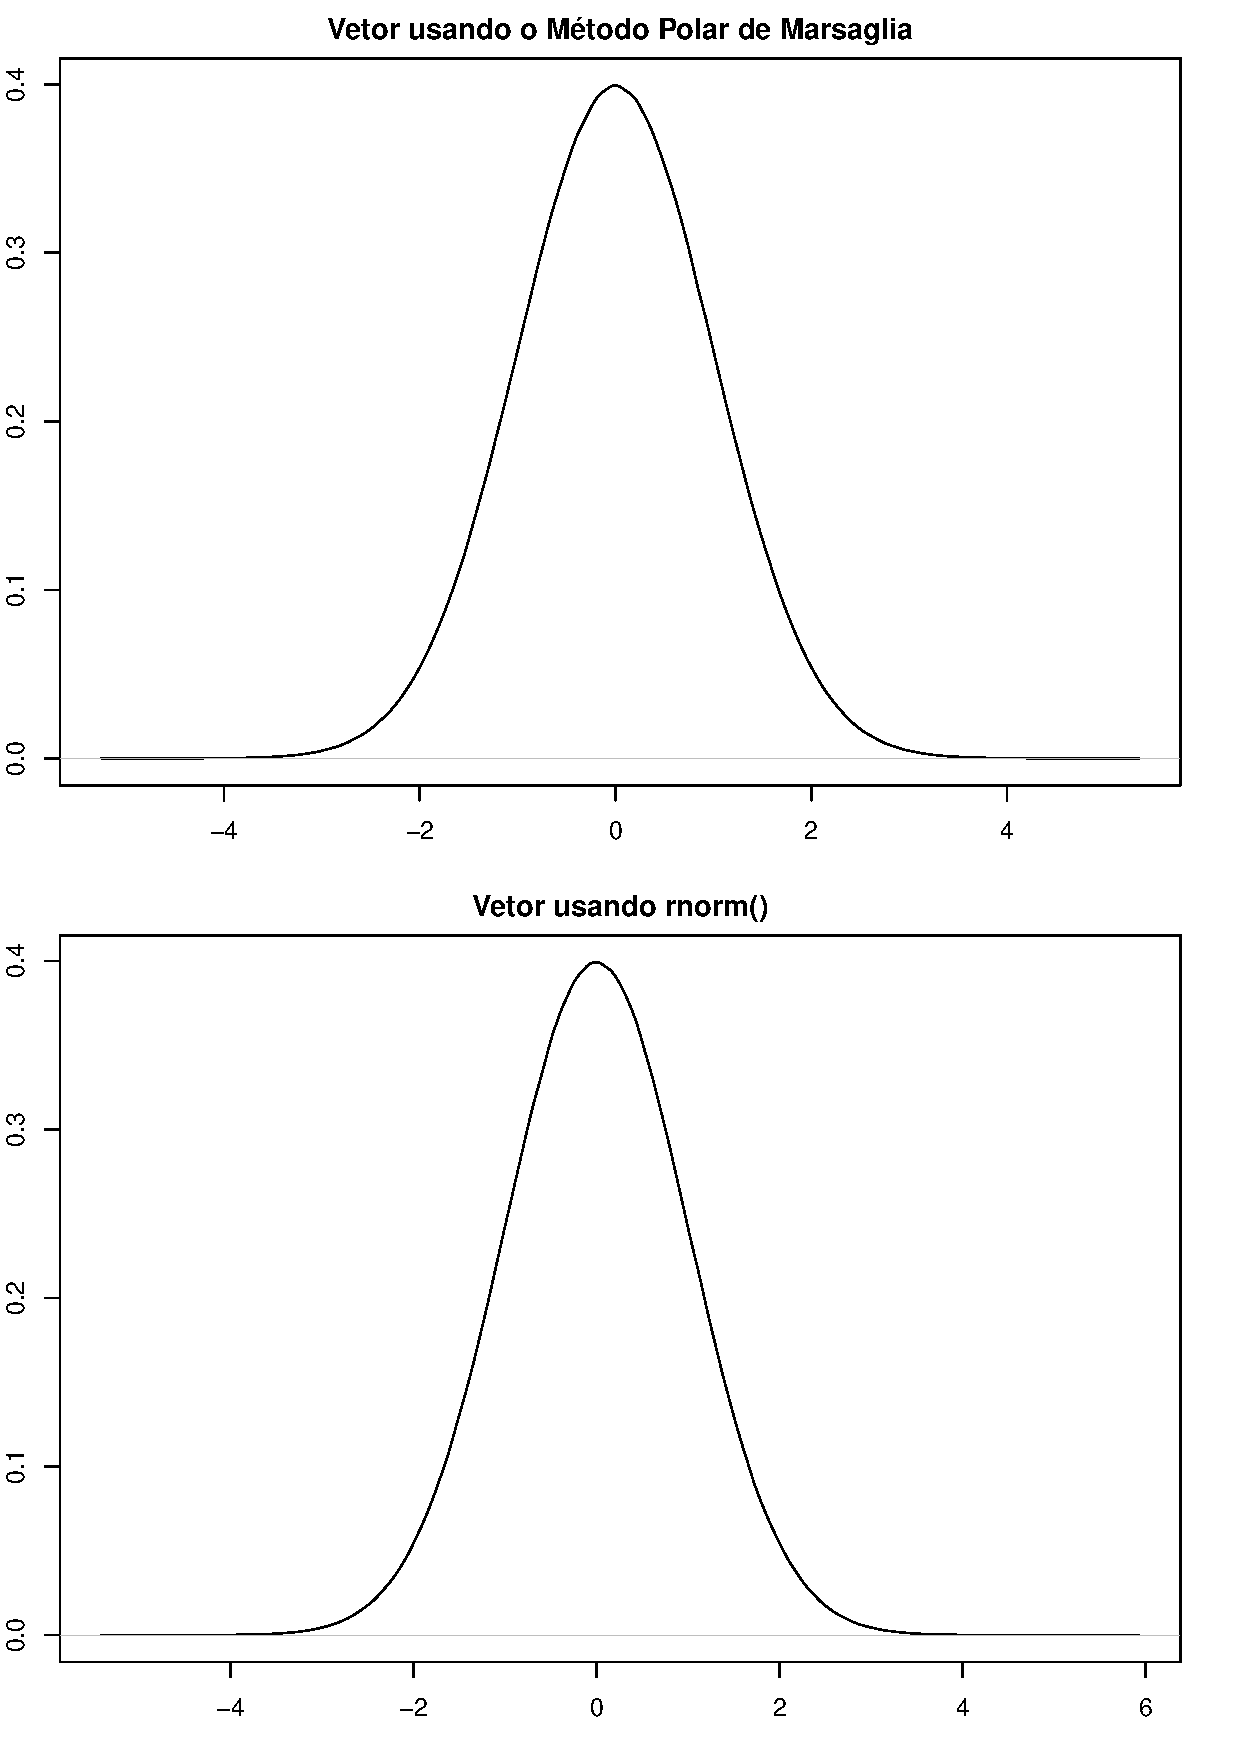
\includegraphics[scale=0.25]{rnorm_polar}
        \caption{Gráficos de Densidade \textit{Kernel} para o gerador que usa o Método Polar de Marsaglia e a para a função rnorm(), $n = 10^7$ em ambos}
        \label{fig:rnorm_polar}
    \end{figure}

    
    	\section{Tabela de densidades acumuladas da Normal(0,1) usando Método de Integração de Monte Carlo}
    	    	
    	As tabelas a seguir fornecem valores para os percentis (0,b) da Normal Padrão, ou seja, cada célula contém o valor de P(0 < Z < b) com $Z \sim Normal(0,1)$, e entre parênteses, o valor encontrado via MC menos o valor obtido pela pnorm() do R para o respectivo quantil.
%    	\newgeometry{left=0.25mm,bottom=0.12mm,top = 0.23mm,right = 0.2mm}
    	\begin{landscape}
    		
    	

    	\begin{table}\footnotesize\label{tabela:pnorm_MC}
    		\begin{tabular}{c||p{17mm}|p{17mm}|p{17mm}|p{17mm}|p{17mm}|p{17mm}|p{17mm}|p{17mm}|p{17mm}|p{17mm}|p{17mm}|p{17mm}|p{17mm}|p{17mm}|p{17mm}|p{17mm}|p{17mm}}
    			~   & .00 & .01 & .02 & .03 & .04 & .05 & .06 & .07 & .08 & .09\\
    			\hline \hline
   			    0.0 & 0.500000 (0.00e+00) & 0.503989 \newline(-4.95e-11)& 0.507978 \newline(-3.96e-10)& 0.511966 \newline(-1.34e-09) & 0.515953 \newline(-3.17e-09) & 0.519939 \newline(6.18e-09) & 0.523922 \newline(-1.07e-08)& 0.527903 \newline(-1.70e-08)& 0.531881 \newline(-2.53e-08)& 0.535856 \newline(-3.60e-08)\\
   			    \hline
    			0.1 & 0.539828\newline(-7.13e-08)&0.543795\newline(-9.49e-08) &0.547758\newline(-1.23e-07)& 0.551717\newline(-1.56e-07)& 0.555670\newline(-1.95e-07)& 0.559618\newline(-2.40e-07)& 0.563559\newline(-2.91e-07)& 0.567495\newline(-3.49e-07)& 0.561424\newline(-4.14e-07)& 0.575345\newline(-4.87e-07)\\
    			\hline
    			0.2 & 0.579260\newline(-3.42e-07)&0.583166\newline(-3.95e-07)&0.587064\newline(-4.54e-07)&0.590954\newline(-5.19e-07)&0.594835\newline(5.89e-07)&0.598706\newline(-6.65e-07)&0.602568\newline(-7.47e-07)&0.602568\newline(-8.36e-07)&0.610261\newline(-9.31e-07)&0.614092\newline(-1.03e-06)\\
    			\hline
    			0.3 & 0.617912\newline(1.14e-06)&0.621720\newline(1.26e-06)&0.625517\newline(1.38e-06)&0.629301\newline(1.52e-06)&0.633073\newline(1.66e-06)&0.636832\newline(1.81e-06)&0.640578\newline(1.96e-06)&0.644310\newline(2.13e-06)&0.648029\newline(2.30e-06)&0.651733\newline(2.49e-06)\\
    			\hline 
    			0.4 & 0.655427\newline(-4.64e-07)& 0.659103\newline(-4.99e-07)& 0.662763\newline(-5.36e-07)&0.666409\newline(-5.75e-07)& 0.670038\newline(-6.15e-07)& 0.673652\newline(-6.57e-07)& 0.677250\newline(-7.01e-07)& 0.680831\newline(-7.47e-07)&0.684395\newline(-7.95e-07)& 0.687942\newline(-8.45e-07) \\
    			\hline 
    			0.5 & 0.691453\newline(-2.13e-06)&0.694965\newline(-2.27e-06)&0.698458\newline(-2.41e-06)&0.701933\newline(-2.56e-06)&0.705390\newline(-2.71e-06)&0.708828\newline(-2.87e-06)&0.712248\newline(-3.04e-06)&0.715648\newline(-3.21e-06)& 0.719029\newline(-3.39e-06)&0.722390\newline(-3.58e-06)\\
    			\hline\hline 
    			0.6 & 0.725735\newline(-1.33e-05) & 0.729057 \newline (-1.39e-05) & 0.732358 \newline (-1.46e-05) & 0.735639 \newline (-1.53e-05) & 0.738900 \newline (-1.60e-05) & 0.742139 \newline (-1.67e-05) & 0.745358 \newline (-1.74e-05) & 0.748555 \newline (-1.82e-05) & 0.751731 \newline (-1.90e-05) & 0.754886 \newline (-1.97e-05)\\
    			\hline 
    			0.7 & 0.758042\newline (-3.35e-05) & 0.761153\newline (-3.48e-05) & 0.764243\newline (-3.62e-05)& 0.767311 \newline (-3.76e-05)& 0.770356\newline (-3.90e-05)& 0.773379 \newline (-4.05e-05) & 0.776379\newline (-4.19e-05) &0.779357\newline (-4.34e-05)& 0.782312\newline(-4.50e-05)& 0.785244\newline(-4.65e-05)\\
    			\hline		
    			
    			0.8 & 0.788137\newline (5.09e-05) & 0.791022 \newline (5.26e-05) & 0.793884 \newline (5.45e-05) & 0.796722 \newline (5.63e-05) & 0.799537\newline (5.82e-05) & 0.802329 \newline (6.01e-05) & 0.805096 \newline(6.20e-05) & 0.807840 \newline (6.40e-05) & 0.810561\newline (6.60e-05)& 0.813257 \newline (6.81e-05)\\
    			
    			\hline
    	
    			0.9 & 0.815915 \newline (-1.78e-05)& 0.818563 \newline (-1.84e-05)& 0.821187 \newline (-1.90e-05) &0.823787\newline(-1.95e-05)& 0.826363\newline (-2.01e-05) & 0.828915 \newline (-2.07e-05)& 0.831442\newline (-2.13e-05)& 0.833946"\newline(-2.19e-05) & 0.836425\newline (-2.26e-05) &0.838880\newline (-2.32e-05)\\
    			\hline\hline
    			1.0 & 0.841236\newline(6.85e-05)& 0.843641\newline(7.03e-05)& 0.846022\newline(7.21e-05)& 0.848378\newline(7.40e-05)& 0.850710\newline(7.59e-05)& 0.853018\newline(7.78e-05)& 0.855302\newline(7.97e-05)& 0.857562\newline(8.17e-05)& 0.859797\newline(8.37e-05)& 0.862009\newline(8.57e-05)\\
    			\hline
    			1.1 & 0.864367\newline(6.11e-05)& 0.866534\newline(6.25e-05)& 0.868677\newline(6.38e-05)& 0.870797\newline(6.52e-05)& 0.872892\newline(6.66e-05)& 0.874964\newline(6.80e-05)& 0.877012\newline(6.94e-05)& 0.879037\newline(7.08e-05)& 0.881038\newline(7.22e-05)& 0.883016\newline(7.37e-05)\\
    			\hline
    			
    			1.2&0.884832 \newline(-9.83e-05)&0.88676 \newline(0.00183)&0.888665 \newline(0.003735)&0.890547 \newline(0.005616)&
0.892405 \newline(0.007475)&
0.894241 \newline(0.009311)&
0.896054 \newline(0.011123)&0.897844 \newline(0.012913)&0.899611 \newline(0.014681)&0.901356 \newline(0.016426)\\
\hline
    			1.3 & 0.903219 \newline(1.99e-05)&0.904922 \newline(1.72e-03)&0.906603 \newline(3.40e-03)&0.908262 \newline(5.06e-03)&0.909898 \newline(6.70e-03)&0.911513 \newline(8.31e-03)&0.913107 \newline(9.91e-03)&0.914679 \newline(0.011479)&0.916229 \newline(1.30e-02)&0.917758 \newline(1.46e-02)\\
    			\hline
    			1.4 & 0.919273 \newline(3.01e-05)&0.920761 \newline(1.52e-03)&0.922227 \newline(2.98e-03)&0.923673 \newline(4.43e-03)& 0.925098\newline(0.005855)&0.926503 \newline(7.26e-03)&0.927888 \newline(0.008645)&0.929253 \newline(1.00e-02)&0.930597 \newline(1.14e-02)&0.931922 \newline(1.27e-02)\\
    			\hline
    			1.5 & 0.933274 \newline(0.000081)&0.934561 \newline(1.37e-03)&0.935828 \newline(2.64e-03)&0.937077 \newline(3.88e-03)&0.938306 \newline(5.11e-03)&0.939517 \newline(6.32e-03)&0.940709 \newline(7.52e-03)&0.941883 \newline(8.69e-03)&0.943039 \newline(9.85e-03)&0.944176 \newline(1.10e-02)\\
    			\hline
    			1.6 & 0.945156 \newline(-4.47e-05)&0.946256 \newline(1.05e-03)&0.947338 \newline(2.14e-03)&0.948402 \newline(3.20e-03)&0.949449\newline(0.004249)&0.95048\newline(5.28e-03)&0.951493 \newline(6.29e-03)&0.95249 \newline(7.29e-03)&0.95347 \newline(8.27e-03)&0.954434 \newline(9.23e-03)\\
    			\hline
    		\end{tabular}
    		\caption{Densidade acumulada da Normal(0,1) em $(0,b)$ obtida via Método de Integração de Monte Carlo. Nos parênteses, o valor encontrado via MC menos o valor obtido pela pnorm() do R para o respectivo quantil}
		\end{table}
		
		\begin{table}\footnotesize
		\begin{tabular}{c||p{18mm}|p{18mm}|p{18mm}|p{18mm}|p{18mm}|p{18mm}|p{18mm}|p{18mm}|p{18mm}|p{18mm}|p{18mm}|p{18mm}|p{18mm}|p{18mm}|p{18mm}|p{18mm}|p{18mm}}
    			1.7 & 0.95544 \newline(5.27e-06)&0.956372 \newline(9.38e-04)&0.957289 \newline(1.85e-03)&0.95819 \newline(2.76e-03)&0.959075 \newline(3.64e-03)&0.959946 \newline(4.51e-03)&0.960801 \newline(5.37e-03)&0.961641 \newline(6.21e-03)&0.962467 \newline(7.03e-03)&0.963278 \newline(7.84e-03)\\
    			\hline
    			1.8 & 0.963982 \newline(-8.72e-05)&0.964764 \newline(0.000694)&0.965532 \newline(1.46e-03)&0.966285 \newline(2.22e-03)&0.967025 \newline(2.96e-03)&0.967752 \newline(3.68e-03)&0.968465 \newline(4.40e-03)&0.969165 \newline(5.10e-03)&0.969852 \newline(5.78e-03)&0.970526 \newline(6.46e-03)\\
    			\hline
    			1.9 &0.971561\newline(0.000278)&0.972214\newline(0.000930)&0.972854\newline(0.001571)&0.973482\newline(0.002199)&0.974098\newline(0.002815)&0.974702\newline(0.003419)&0.975295\newline(0.004012)&0.975876\newline(0.004593)&0.976446\newline(0.005163)&0.977005\newline(0.005721)\\\hline\hline
    			2.0 & 0.977237\newline(-1.28e-05)&0.977771\newline(5.22e-04)&0.978295\newline(1.05e-03)&0.978809\newline(1.56e-03)&0.979311\newline(2.06e-03)&0.979804\newline(2.55e-03)&0.980287\newline(3.04e-03)&0.98076\newline(3.51e-03)&0.981223\newline(3.97e-03)&0.981677\newline(4.43e-03)\\\hline
    			2.1 &0.982103\newline(-3.28e-05)&0.982537\newline(4.02e-04)&0.982963\newline(8.28e-04)&0.98338\newline(1.24e-03)&0.983788\newline(1.65e-03)&0.984187\newline(2.05e-03)&0.984578\newline(2.44e-03)&0.98496\newline(2.82e-03)&0.985334\newline(0.003199)&0.9857\newline(3.56e-03)\\\hline
    			2.2 &0.986247\newline(0.000151)&0.986601\newline(0.000504)&0.986946\newline(0.000850)&0.987284\newline(0.001188)&0.987615\newline(0.001518)&0.987938\newline(0.001841)&0.988254\newline(0.002158)&0.988563\newline(0.002467)&0.988866\newline(0.002769)&0.989161\newline(0.003065)\\\hline
    			2.3 &0.989135\newline(-0.00014)&0.989414\newline(0.000138)&0.989687\newline(0.000411)&0.989954\newline(0.000678)&0.990214\newline(0.000938)&0.990469\newline(0.001193)&0.990718\newline(0.001442)&0.99096\newline(1.68e-03)&0.991198\newline(1.92e-03)&0.991429\newline(2.15e-03)\\\hline
    			2.4 &0.991659\newline(-0.00014)&0.991879\newline(0.000077)&0.992094\newline(2.92e-04)&0.992304\newline(5.02e-04)&0.992509\newline(7.06e-04)&0.992709\newline(9.06e-04)&0.992903\newline(1.10e-03)&0.993094\newline(1.29e-03)&0.993279\newline(1.48e-03)&0.99346\newline(0.001657)\\\hline
    			
    			2.5 &0.993762\newline(-2.87e-05)&0.993936\newline(1.46e-04)&0.994106\newline(3.15e-04)&0.994272\newline(4.81e-04)&0.994433\newline(6.43e-04)&0.994591\newline(0.000801)&0.994745\newline(9.54e-04)&0.994894\newline(1.10e-03)&0.995041\newline(1.25e-03)&0.995183\newline(1.39e-03)\\\hline
    			2.6 & 0.994795\newline(-0.000544)&0.994927\newline(-0.000412)&0.995056\newline(-0.000283)&0.995181\newline(-0.000158)&0.995303\newline(-3.59e-05)&0.995422\newline(8.28e-05)&0.995537\newline(1.98e-04)&0.99565\newline(3.11e-04)&0.995759\newline(4.20e-04)&0.995866\newline(5.27e-04)\\\hline
    			2.7 &0.997312\newline( 7.79e-04)&0.997419\newline(8.86e-04)&0.997524\newline(0.000991)&0.997625\newline(0.001092)&0.997724\newline(0.001191)&0.997821\newline(0.001288)&0.997914\newline(0.001381)&0.998006\newline(0.001473)&0.998095\newline(0.001562)&0.998182\newline(0.001649)\\\hline
    			2.8 &0.997993\newline( 5.48e-04)&0.998072\newline( 6.27e-04)&0.998148\newline(7.03e-04)&0.998223\newline(0.000778)&0.998295\newline(0.000850)&0.998366\newline(0.000921)&0.998434\newline(0.000989)&0.998501\newline(0.001056)&0.998565\newline(0.001120)&0.998628\newline(0.001183)\\\hline
    			2.9 &0.997888\newline(-0.000246)&0.997945\newline(-0.000190)&0.997999\newline(-0.000135)&0.998053\newline(-8.16e-05)&0.998104\newline(-3.00e-05)&0.998154\newline(2.00e-05)&0.998203\newline(6.84e-05)&0.99825\newline(1.15e-04)&0.998295\newline(1.61e-04)&0.998339\newline(2.05e-04)\\\hline
    			3.0 &0.99867\newline(2.03e-05)&0.998713\newline(6.28e-05)&0.998754\newline(1.04e-04)&0.998794\newline(1.44e-04)&0.998833\newline(1.83e-04)&0.99887\newline(2.20e-04)&0.998907\newline(2.56e-04)&0.998942\newline(2.92e-04)&0.998976\newline(3.26e-04)&0.999009\newline(3.59e-04)\\\hline
    			3.1 &1.00007\newline(0.001039)&1.00011\newline(0.001074)&1.00014\newline(0.001107)&1.00017\newline(0.001140)&1.0002\newline(0.001172)&1.00023\newline(0.001202)&1.00026\newline(0.001232)&1.00029\newline(0.00126)&1.00032\newline(0.00129)&1.00035\newline(0.00132)\\\hline
    			3.2 &0.999571\newline(2.58e-04)&0.999596\newline(2.83e-04)&0.99962\newline(0.000307)&0.999644\newline(0.000331)&0.999667\newline(0.000354)&0.999689\newline(0.000376)&0.99971\newline(0.000397)&0.999731\newline(0.000418)&0.999751\newline(0.000438)&0.99977\newline(0.000458)\\\hline
    			

\end{tabular}
\caption{Densidade acumulada da Normal(0,1) em $(0,b)$ obtida via Método de Integração de Monte Carlo. Nos parênteses, o valor encontrado via MC menos o valor obtido pela pnorm() do R para o respectivo quantil (continuação)}
\end{table}

\begin{table}\footnotesize
	\begin{tabular}{c||p{18mm}|p{18mm}|p{18mm}|p{18mm}|p{18mm}|p{18mm}|p{18mm}|p{18mm}|p{18mm}|p{18mm}|p{18mm}|p{18mm}|p{18mm}|p{18mm}|p{18mm}|p{18mm}|p{18mm}}
  				3.3 &0.998938\newline(-0.000579)&0.998952\newline(-0.000564)&0.998966\newline(-0.000551)&0.998979\newline(-0.000538)&0.998992\newline(-0.000525)&0.999004\newline(-0.000513)&0.999016\newline(-0.000501)&0.999027\newline(-0.000490)&0.999037\newline(-0.000479)&0.999048\newline(-0.000469)\\\hline
    			3.4 &0.999377\newline(-0.000286)&0.999389\newline(-0.000274)&0.999399\newline(-0.000264)&0.99941\newline(-0.000253)&0.99942\newline(-0.000243)&0.99943\newline(-0.000233)&0.999439\newline(-0.000224)&0.999448\newline(-0.000215)&0.999457\newline(-0.000207)&0.999465\newline(-0.000198)\\\hline
    			3.5 &0.999125\newline(-0.000642)&0.999133\newline(-0.000635)&0.99914\newline(-0.000628)&0.999147\newline(-0.000621)&0.999153\newline(-0.000614)&0.999159\newline(-0.000608)&0.999165\newline(-0.000602)&0.999171\newline(-0.000596)&0.999177\newline(-0.000591)&0.999182\newline(-0.000586)\\\hline
    			3.6 &1.00103\newline(0.00119)&1.00104\newline(0.00120)&1.00105\newline(0.00121)&1.00106\newline(0.00122)&1.00107\newline(0.00123)&1.00108\newline(0.00124)&1.00109\newline(0.00125)&1.0011\newline(0.00126)&1.00111\newline(0.00127)&1.00112\newline(0.00127)\\\hline
    			3.7 &1.00019\newline(0.000297)&1.00019\newline(0.000301)&1.0002\newline(0.000305)&1.0002\newline(0.000310)&1.00021\newline(0.000313)&1.00021\newline(0.000317)&1.00021\newline(0.000321)&1.00022\newline(0.000325)&1.00022\newline(0.000328)&1.00022\newline(0.000331)\\\hline
    			3.8 &0.999315\newline(-0.000613)&0.999316\newline(-0.000612)&0.999317\newline(-0.000611)&0.999318\newline(-0.000610)&0.999319\newline(-0.000609)&0.999319\newline(-0.000608)&0.99932\newline(-0.000608)&0.99932\newline(-0.000607)&0.999321\newline(-0.000607)&0.999321\newline(-0.000606)\\\hline
    			3.9 &0.999732\newline(-0.000220)&0.999733\newline(-0.000219)&0.999735\newline(-0.000217)&0.999736\newline(-0.000216)&0.999737\newline(-0.000215)&0.999738\newline(-0.000214)&0.999739\newline(-0.000213)&0.99974\newline(-0.000212)&0.999741\newline(-0.000211)&0.999742\newline(-0.000210)\\
\end{tabular}
\caption{Densidade acumulada da Normal(0,1) em $(0,b)$ obtida via Método de Integração de Monte Carlo. Nos parênteses, o valor encontrado via MC menos o valor obtido pela pnorm() do R para o respectivo quantil (continuação)}
\end{table}

\end{landscape}
    \section{Tabela de densidades acumuladas da Normal(0,1) usando a Densidade Acumulada Empírica da Transformação Polar de Marsaglia}
    
        	As tabelas a seguir fornecem valores para os percentis (0,b) da Normal Padrão, ou seja, cada célula contém o valor de P(0 < Z < b) com $Z \sim Normal(0,1)$, e entre parênteses, o valor encontrado via Transformação Polar menos o valor obtido pela pnorm() do R para o respectivo quantil.
        	\begin{landscape}
        	\begin{table}\footnotesize\label{tabela:pnorm_polar}
    		\begin{tabular}{c||p{18mm}|p{18mm}|p{18mm}|p{18mm}|p{18mm}|p{18mm}|p{18mm}|p{18mm}|p{18mm}|p{18mm}|p{18mm}|p{18mm}|p{18mm}|p{18mm}|p{18mm}|p{18mm}|p{18mm}}
    			~   & .00 & .01 & .02 & .03 & .04 & .05 & .06 & .07 & .08 & .09\\
    			\hline \hline
    			0.0 &0.50211\newline(0.00211)&0.5059\newline(0.00590)&0.509915\newline(0.00992)&0.51402\newline(0.01402)&0.518225\newline(0.01823)&0.52202\newline(0.02202)&0.52595\newline(0.02595)&0.5298\newline(0.02980)&0.533455\newline(0.03346)&0.53741\newline(0.03741)\\
   			    \hline
    			0.1 & 0.539615\newline(-0.000213)&0.543885\newline(4.06e-03)&0.547805\newline(7.98e-03)&0.551995\newline(0.012167)&0.556\newline(0.01617)&0.559965\newline(0.020137)&0.563855\newline(0.024027)&0.5679\newline(0.028072)&0.57177\newline(0.031942)&0.575645\newline(0.03582)\\
    			\hline
    			0.2 & 0.57933\newline(7.03e-05)&0.58321\newline(3.95e-03)&0.587185\newline(0.007925)&0.59092\newline(1.17e-02)&0.594985\newline(0.01573)&0.599035\newline(0.019775)&0.60298\newline(0.023720)&0.606835\newline(0.027575)&0.6109\newline(0.031640)&0.61476\newline(0.035500)\\
    			\hline
    			0.3 & 0.6168\newline(-0.00111)&0.620305\newline(0.00239)&0.62406\newline(0.00615)&0.62796\newline(0.01005)&0.63181\newline(0.01390)&0.6356\newline(0.01769)&0.6394\newline(0.02149)&0.64314\newline(0.02523)&0.64702\newline(0.02911)&0.65086\newline(0.032949)\\
    			\hline 
    			0.4 & 0.65609\newline(0.000668)&0.659765\newline(0.004343)&0.66359\newline(0.008168)&0.667305\newline(0.011883)&0.67067\newline(0.015248)&0.67425\newline(0.018828)&0.67782\newline(0.022398)&0.681515\newline(0.026093)&0.68494\newline(0.029518)&0.68843\newline(0.033008)\\
    			\hline 
    			0.5 & 0.691965\newline(0.000503)&0.69548\newline(0.004018)&0.69895\newline(0.007488)&0.70226\newline(0.010798)&0.70561\newline(0.014148)&0.70899\newline(0.01753)&0.71255\newline(0.02109)&0.716215\newline(0.024753)&0.71964\newline(0.028178)&0.722945\newline(0.03148)\\
    			\hline\hline 
    			0.6 & 0.72452\newline(-0.00123)&0.72782\newline( 0.00207)&0.731275\newline( 0.00553)&0.734715\newline(0.008968)&0.73792\newline(0.012173)&0.74133\newline(0.015583)&0.74458\newline(0.018833)&0.7478\newline(0.022053)&0.75095\newline(0.025203)&0.754075\newline(0.028328)\\
    			\hline 
    			0.7 & 0.757555\newline(-0.000481)&0.760655\newline(0.002619)&0.76368\newline(0.005644)&0.76657\newline(0.008534)&0.76955\newline(0.01151)&0.77277\newline(0.014734)&0.775645\newline(0.017609)&0.778625\newline(0.020589)&0.781465\newline(0.02343)&0.78418\newline(0.02614)\\
    			\hline		
    			
    			0.8 & 0.78875\newline(0.000605)&0.79151\newline(0.00337)&0.79447\newline(0.006325)&0.797215\newline(0.009070)&0.799785\newline(0.011640)&0.80253\newline(0.014385)&0.805245\newline(0.01710)&0.80788\newline(1.97e-02)&0.810395\newline(0.022250)&0.81328\newline(2.51e-02)\\
    			
    			\hline
    	
    			0.9 & 0.81577\newline(-0.00017)&0.818465\newline(0.002525)&0.82102\newline(0.005080)&0.823585\newline(0.007645)&0.82631\newline(1.04e-02)&0.828825\newline(0.012885)&0.83143\newline(1.55e-02)&0.834105\newline(0.018165)&0.83657\newline(0.020630)&0.83902\newline(0.023080)\\
    			\hline\hline
    			1.0 &0.841835\newline(0.00049)&0.84418\newline(0.002835)&0.846525\newline(0.005180)&0.848925\newline(0.00758)&0.85132\newline(0.00998)&0.85382\newline(0.012475)&0.85613\newline(0.014785)&0.85844\newline(0.01710)&0.860725\newline(0.019380)&0.862755\newline(0.021410)\\
    			\hline
    			1.1 & 0.865295\newline(0.000961)& 0.86741\newline(0.00308)&0.869395\newline(0.005061)&0.871665\newline(0.007331)&0.8738\newline(0.009466)&"0.87585\newline(0.011516)&0.877935\newline(0.013601)&0.87975\newline(0.01542)&0.88159\newline(0.01726)&0.8836\newline(0.019266)\\
    			\hline
    			
    			1.2& 0.884855\newline(-7.53e-05)&0.886775\newline(1.84e-03)&0.88869\newline(3.76e-03)&0.89043\newline(0.005500)&0.892165\newline(0.007235)&0.89397\newline(0.00904)&0.89586\newline(0.010930)&0.897665\newline(0.012735)&0.89931\newline(0.014380)&0.90109\newline(0.016160)\\
\hline
    			1.3 & 0.90415\newline(0.000950)&0.905985\newline(0.002785)&0.90763\newline(0.004430)&0.9093\newline(0.006100)&0.91108\newline(0.007880)&0.91249\newline(0.009290)&0.91414\newline(0.010940)&0.915575\newline(0.012375)&0.917055\newline(0.013855)&0.91877\newline(0.01557)\\
    			\hline
    			1.4 & 0.919235\newline(-8.34e-06)&0.92072\newline(1.48e-03)&0.922175\newline(2.93e-03)&0.923545\newline(4.30e-03)&0.925075\newline(5.83e-03)&0.92648\newline(7.24e-03)&0.928045\newline(0.00880)&0.92946\newline(0.010217)&0.930965\newline(0.011722)&0.93231\newline(0.013067)\\
    			\hline
    			1.5 & 0.93331\newline(0.000117)&0.93457\newline(1.38e-03)&0.93585\newline(0.002657)&0.937165\newline(0.003972)&0.938455\newline(0.005262)&0.93956\newline(0.006367)&0.9406\newline(7.41e-03)&0.941745\newline(8.55e-03)&0.94284\newline(0.009647)&0.944\newline(1.08e-02)\\
    			\hline
    			1.6 & 0.94567\newline(0.000469)&0.94674\newline(0.001539)&0.947855\newline(0.002654)&0.948955\newline(0.003754)&0.950085\newline(0.004884)&0.95115\newline(0.005949)&0.952155\newline(0.006954)&0.953145\newline(0.007944)&0.95417\newline(0.008969)&0.95523\newline(0.010029)\\
    			\hline
        		\end{tabular}
        		\caption{Densidade acumulada da Normal(0,1) em $(0,b)$ obtida via Transformação Polar de Marsaglia. Nos parênteses, o valor encontrado via Transformação Polar menos o valor obtido pela pnorm() do R para o respectivo quantil (continuação)}
        	\end{table}


		\begin{table}\footnotesize
		\begin{tabular}{c||p{18mm}|p{18mm}|p{18mm}|p{18mm}|p{18mm}|p{18mm}|p{18mm}|p{18mm}|p{18mm}|p{18mm}|p{18mm}|p{18mm}|p{18mm}|p{18mm}|p{18mm}|p{18mm}|p{18mm}}
		    			~   & .00 & .01 & .02 & .03 & .04 & .05 & .06 & .07 & .08 & .09\\
    			\hline \hline
    			1.7 & 0.95542\newline(-1.45e-05)&0.95647\newline(0.001035)&0.95742\newline(0.001985)&0.95841\newline(0.002975)&0.9593\newline(0.003865)&"0.960205\newline(0.004770)&0.96108\newline(0.005645)&0.96186\newline(0.006425)&0.96256\newline(0.007125)&0.963295\newline(0.007860)\\
    			\hline
    			1.8 & 0.96358\newline(-0.00049)&0.96437\newline(0.000300)&0.965235\newline(0.001165)&0.965915\newline(0.001845)&0.96673\newline(0.002660)&0.96751\newline(0.003440)&0.968255\newline(0.004185)&0.96901\newline(0.004940)&0.969705\newline(0.005635)&0.970385\newline(0.006315)\\
    			\hline
    			1.9 &0.97167\newline(0.000387)&0.97223\newline(0.000947)&0.972915\newline(0.001632)&0.97354\newline(0.002257)&0.974085\newline(0.002802)&0.974665\newline(0.003382)&0.975365\newline(0.004082)&0.97596\newline(0.004677)&0.97656\newline(0.005277)&0.977155\newline(0.00587)\\\hline\hline
    			2.0 & 0.977155\newline(-9.49e-05)&0.977745\newline(4.95e-04)&0.978355\newline(1.11e-03)&0.978915\newline(1.67e-03)&0.97939\newline(2.14e-03)&0.979885\newline(2.64e-03)&0.980465\newline(0.003215)&0.980895\newline(0.003645)&0.98141\newline(0.004160)&0.981805\newline(0.004555)\\\hline
    			2.1 &0.982115\newline(-2.06e-05)&0.982625\newline(4.89e-04)&0.983015\newline(0.000879)&0.983445\newline(1.31e-03)&0.983825\newline(1.69e-03)&0.984265\newline(2.13e-03)&0.98464\newline(2.50e-03)&0.98497\newline(2.83e-03)&0.98534\newline(3.20e-03)&0.985725\newline(3.59e-03)\\\hline
    			2.2 &0.98602\newline(-7.66e-05)&0.986375\newline(2.78e-04)&0.98668\newline(0.000583)&0.98703\newline(9.33e-04)&0.987425\newline(1.33e-03)&0.987785\newline(1.69e-03)&0.988095\newline(2.00e-03)&0.988435\newline(2.34e-03)&0.98876\newline(2.66e-03)&0.989095\newline(0.002998)\\\hline
    			2.3 &0.98921\newline(-6.59e-05)&0.98954\newline(2.64e-04)&0.98979\newline(5.14e-04)&0.99\newline(7.24e-04)&0.990255\newline(0.000979)&0.990585\newline(1.31e-03)&0.99079\newline(1.51e-03)&0.99104\newline(0.001764)&0.991265\newline(1.99e-03)&0.991495\newline(2.22e-03)\\\hline
    			2.4 &0.99188\newline(7.75e-05)&0.992035\newline(2.33e-04)&0.992165\newline(3.63e-04)&0.99236\newline(5.58e-04)&0.99253\newline(7.28e-04)&0.99276\newline(9.58e-04)&0.99295\newline(1.15e-03)&0.99314\newline(1.34e-03)&0.99332\newline(1.52e-03)&0.993485\newline(1.68e-03)\\\hline
    			
    			2.5 &0.993835\newline(4.47e-05)&0.99403\newline(2.40e-04)&0.994215\newline(4.25e-04)&0.99441\newline(6.20e-04)&0.99456\newline(7.70e-04)&0.99475\newline(9.60e-04)&0.994935\newline(1.14e-03)&0.995045\newline(0.001255)&0.995245\newline(1.45e-03)&0.995405\newline(0.001615)\\\hline
    			2.6 & 0.99536\newline(2.12e-05)&0.99547\newline(1.31e-04)&0.995605\newline(2.66e-04)&0.99573\newline(3.91e-04)&0.99584\newline(5.01e-04)&0.99599\newline(6.51e-04)&0.99609\newline(7.51e-04)&0.996235\newline(8.96e-04)&0.99635\newline(1.01e-03)&0.996435\newline(1.10e-03)\\\hline
    			2.7 &0.99658\newline(4.70e-05)&0.99665\newline(1.17e-04)&0.99675\newline(2.17e-04)&0.99691\newline(3.77e-04)&0.99702\newline(4.87e-04)&0.99711\newline(5.77e-04)&0.997185\newline(6.52e-04)&0.99726\newline(7.27e-04)&0.99736\newline(8.27e-04)&0.99743\newline(8.97e-04)\\\hline
    			2.8 &0.99743\newline(-1.49e-05)&0.997545\newline(1.00e-04)&0.997625\newline(1.80e-04)&0.9977\newline(2.55e-04)&0.997755\newline(3.10e-04)&0.997785\newline(3.40e-04)&0.99789\newline(4.45e-04)&0.997985\newline(5.40e-04)&0.998035\newline(5.90e-04)&0.998105\newline(6.60e-04)\\\hline
    			2.9 &0.998035\newline(-9.92e-05)&0.998075\newline(-5.92e-05)&0.998155\newline(2.08e-05)&0.9982\newline(6.58e-05)&0.998265\newline(1.31e-04)&0.998305\newline(1.71e-04)&0.99836\newline(2.26e-04)&0.9984\newline(2.66e-04)&0.998445\newline(3.11e-04)&0.998495\newline(3.61e-04)\\\hline
    			3.0 &0.998545\newline(-0.000105)&0.99859\newline(-6.01e-05)&0.998645\newline(-5.10e-06)&0.99869\newline(3.99e-05)&0.998725\newline(7.49e-05)&0.99879\newline(1.40e-04)&0.998815\newline(1.65e-04)&0.998845\newline(1.95e-04)&0.998905\newline(2.55e-04)&0.99892\newline(2.70e-04)\\\hline
    			3.1 &0.999055\newline(2.26e-05)&0.99908\newline(4.76e-05)&0.999115\newline(8.26e-05)&0.999155\newline(1.23e-04)&0.99919\newline(1.58e-04)&0.999205\newline(1.73e-04)&0.999235\newline(2.03e-04)&0.999265\newline(2.33e-04)&0.999295\newline(2.63e-04)&0.999315\newline(2.83e-04)\\\hline
    			3.2 &0.999365\newline(5.21e-05)&0.999395\newline(8.21e-05)&0.999435\newline(1.22e-04)&0.999445\newline(1.32e-04)&0.999475\newline(1.62e-04)&0.99949\newline(1.77e-04)&0.999505\newline(1.92e-04)&0.999515\newline(2.02e-04)&0.999555\newline(2.42e-04)&0.99956\newline(2.47e-04)\\\hline
    			

\end{tabular}
\caption{Densidade acumulada da Normal(0,1) em $(0,b)$ obtida via Transformação Polar de Marsaglia. Nos parênteses, o valor encontrado via Transformação Polar menos o valor obtido pela pnorm() do R para o respectivo quantil (continuação)}
\end{table}

\begin{table}\footnotesize
	\begin{tabular}{c||p{18mm}|p{18mm}|p{18mm}|p{18mm}|p{18mm}|p{18mm}|p{18mm}|p{18mm}|p{18mm}|p{18mm}|p{18mm}|p{18mm}|p{18mm}|p{18mm}|p{18mm}|p{18mm}|p{18mm}}
	    			~   & .00 & .01 & .02 & .03 & .04 & .05 & .06 & .07 & .08 & .09\\
    			\hline \hline
  				3.3 &0.99954\newline(2.34e-05)&0.99955\newline(3.34e-05)&0.99956\newline(4.34e-05)&0.99957\newline(5.34e-05)&0.99959\newline(7.34e-05)&0.999595\newline(7.84e-05)&0.999605\newline(8.84e-05)&0.999615\newline(9.84e-05)&0.999625\newline(1.08e-04)&0.99963\newline(1.13e-04)\\\hline
    			3.4 &0.999615\newline(-4.81e-05)&0.99963\newline(-3.31e-05)&0.999635\newline(-2.81e-05)&0.999655\newline(-8.07e-06)&0.99966\newline(-3.07e-06)&0.999685\newline(2.19e-05)&0.999685\newline(2.19e-05)&0.99969\newline(2.69e-05)&0.99971\newline(4.69e-05)&0.99972\newline(5.69e-05)\\\hline
    			3.5 &0.999745\newline(-2.24e-05)&0.99975\newline(-1.74e-05)&0.999755\newline(-1.24e-05)&0.99977\newline(2.63e-06)&0.99977\newline(2.63e-06)&0.999775\newline(7.63e-06)&0.99978\newline(1.26e-05)&0.99978\newline(1.26e-05)&0.99979\newline(2.26e-05)&0.999795\newline(2.76e-05)\\\hline
    			3.6 &0.99988\newline( 3.91e-05)&0.999895\newline(5.41e-05)&0.999915\newline(7.41e-05)&0.999915\newline(7.41e-05)&0.999915\newline(7.41e-05)&0.999915\newline(7.41e-05)&0.99993\newline(8.91e-05)&0.99993\newline(8.91e-05)&0.999935\newline(9.41e-05)&0.999935\newline(9.41e-05)\\\hline
    			3.7 &0.999895\newline(2.80e-06)&0.999895\newline(2.80e-06)&0.999895\newline( 2.80e-06)&0.9999\newline(7.80e-06)&0.999915\newline(2.28e-05)&0.999915\newline(2.28e-05)&0.999915\newline(2.28e-05)&0.99992\newline(2.78e-05)&0.999925\newline(3.28e-05)&0.999925\newline(3.28e-05)\\\hline
    			3.8 &0.99995\newline(2.23e-05)&0.999955\newline(2.73e-05)&0.999955\newline(2.73e-05)&0.999955\newline(2.73e-05)&0.99996\newline(3.23e-05)&0.99996\newline(3.23e-05)&0.99996\newline(3.23e-05)&0.99996\newline(3.23e-05)&0.999965\newline(3.73e-05)&0.999965\newline(3.73e-05)\\\hline
    			3.9 &0.999965\newline(1.31e-05)&0.999965\newline( 1.31e-05)&0.999965\newline(1.31e-05)&0.99997\newline(1.81e-05)&0.99997\newline(1.81e-05)&0.99997\newline(1.81e-05)&0.999975\newline(2.31e-05)&0.999975\newline(2.31e-05)&0.999975\newline(2.31e-05)&0.999975\newline(2.31e-05)\\
\end{tabular}
\caption{Densidade acumulada da Normal(0,1) em $(0,b)$ obtida via Transformação Polar de Marsaglia. Nos parênteses, o valor encontrado via Transformação Polar menos o valor obtido pela pnorm() do R para o respectivo quantil (continuação)}

\end{table}
        	\end{landscape}
        	
\section{Conclusões}\label{cap:conclusoes}
\subsection{Sobre o Gerador Congruencial para a Uniforme (0,1)}
	\begin{itemize}
  \item A significância dos testes foi alta, o que significa que o gerador é eficaz em gerar uma amostra da U(0,1).
  \item Comentários sobre a baixa eficiência de implementação de quase todo algoritmo em R sempre serão oportunos, já que o mesmo tem foco maior na legibilidade do código e proximidade com a "linguagem natural" do que com velocidade. Como não foi pedido este tipo de análise do comando do trabalho, decidimos por não estender mais um ainda um trabalho que já ficou longo.
\end{itemize}

\subsection{Sobre o Gerador usando a Transformação Polar de Marsaglia para a Normal (0,1)}
  \begin{itemize}
  \item Importante notar que, como este Gerador utiliza o Gerador Congruencial para U(0,1) implementado aqui, era essencial que os Testes para ambos fossem significativos. E foram.
  \item Foram implementadas duas versões do gerador: uma que utiliza as funções \textbf{sin()} e \textbf{cos()} do próprio R e outra que utiliza a Transformação de Marsaglia. Note que esta segunda é necessariamente mais eficiente que a primeira, já que o cálculo de funções trigonométricas tem um custo não-negligenciável\footnote{Para uma discussão mais substancial sobre o tema, ver \url{http://stackoverflow.com/q/2284860/4965975}}.
\end{itemize}
\subsection{Sobre a tabela de Densidades Acumuladas da Normal(0,1) utilizando Método de Integração de Monte Carlo}

\begin{itemize}
  \item Sob uma ótica qualitativa, entendemos que os resultados foram satisfatórios. Temos uma maioria de diferenças que têm ordem $10^{-6}$, com algumas excentricidades nos quantis a partir de 3, como as densidades acumuladas acima de 1 em 3.1, 3.6 e 3.7. Como estão acima de 1 mas espera-se de qualquer maneira que sejam muito próximas de 1, entendemos que isso não desabona o método.
  \item Uma observação importante sobre a construção da tabela: para fins estéticos, foi utilizada a função \textbf{format()} do R para especificar o número de dígitos do resultado, o que resulta em aproximações. Para o percentil da acumulada (o valor da célula sem os parênteses), foi utilizado o parâmetro \textbf{digits = 6}, ou seja, o 7o dígito foi arredondado. Para os erros (valores entre parênteses na 2a linha da célula), o parâmetro digits teve valor 3, pois o entendimento foi que a ordem de grandeza dos erros era mais relevante que o seu valor em si.
  \item O R utiliza uma implementação do pacote QUADPACK\cite{wiki:003} em C, que por sua vez é uma implementação da Quadratura da Fórmula da Quadratura de Gauss-Kronrod para Integração Numérica, inclusive para \textbf{pnorm()} e similares. A impressão de que a Integração via MC é mais simples que este método é muito clara.
\end{itemize}

\subsection{Sobre a tabela de Densidades Acumuladas da Normal(0,1) utilizando Transformação Polar de Marsaglia}
\begin{itemize}
  \item A implementação da Densidade Acumulada Empírica que foi utilizada para aproximar a Densidade Acumulada é, grosso modo, uma aplicação do Método de Rejeição. Isso resultou numa implementação fácil, mas diminui a robustez do procedimento quando o número de rejeições é muito baixo e há arredondamento.
  \item Em tempo, a construção da tabela foi feita de maneira muito similar à utilizada na tabela usando o Método de Monte Carlo.
  \item Ao contrário do Método de Monte Carlo, o Método Polar não resultou em percentis > 1, justamente pelo fato de ser uma implementação do Método de Rejeição.
\end{itemize}


	
\bibliography{TP2-EstComp.bib}

\section{Anexo A - Códigos das Implementações em R}
Lembrete: repositório completo do Trabalho Prático, inclusive escrita do relatório, em \url{https://github.com/august-o/TP2-EstComp}

\subsection{runif\_congruencial.R}

Implementa o Gerador Congruencial da U(0,1). O objeto .Random.seed é um vetor aleatório gerado pelo R a cada execução do interpretador.
\lstset{language=R,numbers=left,frame=single}
\begin{lstlisting}
runif_congruencial <- function(n = 1) {
  a <- 62089911
  m <- (2 ^ 31) - 1
  x <- c(0)
  y <- c(0)
  x[1] <- 0
  y[1] <- sample(.Random.seed[.Random.seed > 0], 1)
  if (n == 1) {
    y_0 <- y[1]
    y[1] <- (a * y_0) %% m
    x[1] = y[1] / m
  }
  else{
    y_0 <- y[1]
    y[1] <- (a * y_0) %% m
    x[1] = y[1] / m
    for (i in 2:n) {
      y[i] <- (a * y[i - 1]) %% m
      x[i] <- y[i] / m
    }
  }
  return(x)
}
\end{lstlisting}

\subsection{rnorm\_polar.R}
Implementa o gerador usando o Método Polar para a N(0,1). \textbf{rnorm\_polarTrig()} utiliza \textbf{sin()} e \textbf{cos()}, enquanto \textbf{rnorm\_polarDireto()} utiliza as Transformações de Box-Muller/Marsaglia para um procedimento mais eficiente. Para fins de construção da tabela, foi utilizada a opção mais eficiente. 
\begin{lstlisting}
rnorm_polarTrig <- function(n = 1) {
  resultado <- c()
  i <- 1
  while (i <= n) {
    u1 <- runif_congruencial()
    r2 <- -2 * log(u1)
    u2 <- runif_congruencial()
    theta <- 2 * pi * u2
    x <- sqrt(r2) * cos(theta)
    y <- sqrt(r2) * sin(theta)
    resultado <- append(resultado, c(x, y))
    i <- i + 1
  }
  return(resultado)
}

rnorm_polarDireto <- function(n=1){
  X <- matrix(0, ncol = 2, nrow = n)
  for (i in 1:n){
    U <- runif(2)
    V <- 2 * U - 1
    R2 <- sum(V^2)
    while (R2 > 1){
      U <- runif(2)
      V <- 2 * U - 1
      R2 <- sum(V^2)
    }
    Y <- sqrt(-2 * log(R2) / R2)
    X[i, ] <- Y * V
  }
  as.vector(X)
}
\end{lstlisting}

\subsection{pnorm\_MC.R}
Implementa o Método de Integração de Monte Carlo para obter uma aproximação para a Densidade Acumulada da N(0,1) na forma $P(0<Z<b)$. 

\textbf{NOTA}: Como este código foi utilizado para redigir o trabalho, o retorno da função é uma lista com o valor encontrado para fda usando MC e caracteres especiais do Latex que auxiliaram na construção da tabela, seguido pela diferença entre o valor via MC e via pnorm() do R.

\begin{lstlisting}
pnorm_MC <- function(x, n = 10^6){
  t <- runif(n)
  fda <- numeric(length(x))
  resultado <- list(length(x))
  for(i in 1:length(x)){
    g <- x[i]*exp(-0.5*(x[i]*t)^2)
    fda[i] <- mean(g)/sqrt(2*pi) + 0.5
    resultado[i] <- paste(format(fda[i],digits = 6),"
    \newline(",format(fda[i]-pnorm(x),digits=3),")&",sep="")
  }
  return(resultado)
}
\end{lstlisting}

\subsection{pnorm\_polar.R}
Implementa uma aproximação para a Densidade Acumulada da N(0,1) utilizando Transformação Polar de Marsaglia e Método da Rejeição. Ver \textbf{NOTA} acima para explicação sobre o retorno da função.

\begin{lstlisting}
	pnorm_polar <- function(x,n=10^5){
  resultado <- list(length(x))
  fda <- numeric(length(x))
  t <- rnorm_polarDireto(n)
  mean(ifelse(t<x,1,0))
  for(i in 1:length(x)){
    fda[i] <- mean(ifelse(t<x[i],1,0))
    resultado[i] <- paste(format(fda[i],digits = 6),
    "\newline(",format(fda[i]-pnorm(x),digits=3),")&",sep="")
  }
  return(resultado)
\end{lstlisting}




\end{document}
